%
% introduction.tex
%
% Copyright (C) 2020 by SpaceLab.
%
% EPS 2.0 Documentation
%
% This work is licensed under the Creative Commons Attribution-ShareAlike 4.0
% International License. To view a copy of this license,
% visit http://creativecommons.org/licenses/by-sa/4.0/.
%

%
% \brief Introduction chapter.
%
% \author Gabriel Mariano Marcelino <gabriel.mm8@gmail.com>
%
% \institution Universidade Federal de Santa Catarina (UFSC)
%
% \version 0.1.0
%
% \date 2020/11/05
%

\chapter{Introduction} \label{ch:introduction}

The Electrical Power System (EPS\nomenclature{\textbf{EPS}}{\textit{Electric Power System.}}) has been designed to harvest, store and distribute energy for a CubeSat. The energy harvesting system is based on solar energy conversion through six solar panels attached to the CubeSat structure. The EPS is designed to operate the solar panels at their maximum power point. The harvested solar energy is stored in the battery module connected to the EPS. The energy distribution is done by several integrated DC-DC converters. The full EPS system is composed of the solar panels, the EPS PCB and the battery module. A general view of the EPS 2.0 board can be seen in \autoref{fig:general-view}.

\begin{figure}[!ht]
    \begin{center}
        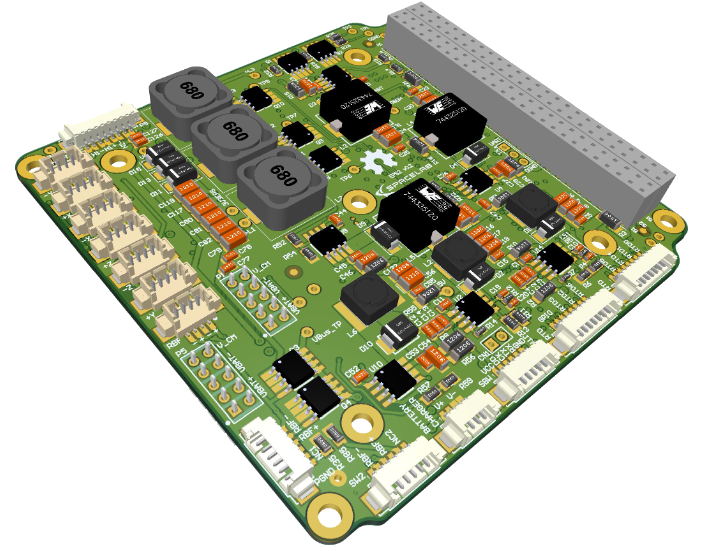
\includegraphics[width=0.75\textwidth]{figures/eps2-pcb-3d}
        \caption{3D view of the EPS 2.0 PCB.}
        \label{fig:general-view}
    \end{center}
\end{figure}

The main characteristics of the EPS module are available below:

\begin{itemize}
    \item Compatible with Gomspace Solar Panels or panel of similar characteristics.
    \item Compliant with CubeSat standard.
    \item Low power MSP430 MCU \@ 20 MHz.
    \item Maximum power point tracking (MPPT).
    \item Overvoltage, undervoltage, overcurrent and short circuit protection for the battery module.
    \item Consumption measurement capability.
    \item Solar panels power measurement capability.
    \item Battery module measurements capability.
    \item 3.3V/1A (x1), 3.3V/2A (x2), 5V/3A (x1), 5V/5A (x2) and one battery voltage supply output pins.
    \item Seven temperature measurements with high accuracy.
    \item Low power operation capability.
\end{itemize}

\cite{test}, \cite{obdh2}
